% EvoClaw TikZ Figures — Standalone compilation
% Compile with: pdflatex evoclaw-tikz-figures.tex
%
% These figures are embedded inline in evoclang-paper-enhanced.tex
% This file provides standalone versions for separate compilation/preview.

\documentclass[border=10pt]{standalone}
\usepackage{tikz}
\usepackage{pgfplots}
\usepackage[T1]{fontenc}
\usepackage[utf8]{inputenc}

\usetikzlibrary{arrows.meta, positioning, shapes.geometric, shapes.multipart,
  fit, calc, decorations.pathreplacing, backgrounds, shadows.blur,
  patterns, chains, matrix}

\pgfplotsset{compat=1.18}

% Color palette
\definecolor{coreblue}{HTML}{2563EB}
\definecolor{coreteal}{HTML}{0D9488}
\definecolor{coreorange}{HTML}{EA580C}
\definecolor{corepurple}{HTML}{7C3AED}
\definecolor{coregray}{HTML}{64748B}
\definecolor{coregreen}{HTML}{16A34A}
\definecolor{corered}{HTML}{DC2626}
\definecolor{lightbg}{HTML}{F8FAFC}
\definecolor{edgebg}{HTML}{ECFDF5}
\definecolor{serverbg}{HTML}{EFF6FF}
\definecolor{cloudbg}{HTML}{FEF3C7}

\begin{document}

%% ========================================================================
%%  FIGURE 1: System Architecture
%% ========================================================================

\begin{tikzpicture}[
    >=Stealth,
    node distance=0.6cm and 1.2cm,
    layer/.style={draw, rounded corners=4pt, minimum width=12.5cm, minimum height=1.8cm, fill=#1, font=\small},
    component/.style={draw, rounded corners=3pt, minimum width=2.5cm, minimum height=0.9cm, fill=white, font=\footnotesize, drop shadow={shadow xshift=0.5pt, shadow yshift=-0.5pt, opacity=0.15}},
    mqttbox/.style={draw, rounded corners=3pt, minimum width=12.5cm, minimum height=0.9cm, fill=coreteal!10, font=\footnotesize\bfseries, draw=coreteal!60},
    arrow/.style={->, thick, color=coregray},
    biarrow/.style={<->, thick, color=coreteal},
    label/.style={font=\footnotesize\bfseries, color=#1},
]

% Layer 1: Orchestrator
\node[layer=serverbg, label={[label=coreblue]above left:{Layer 1: Go Orchestrator}}] (orch) at (0, 4.5) {};
\node[component] (api) at (-4.2, 4.5) {REST API\\(Gin)};
\node[component] (ws) at (-1.4, 4.5) {WebSocket\\Gateway};
\node[component] (director) at (1.8, 4.5) {Director\\Engine};
\node[component] (mutator) at (4.8, 4.5) {Genome\\Mutator};

% Layer 2: MQTT
\node[mqttbox] (mqtt) at (0, 3.0) {MQTT Broker (Mosquitto) --- Topics: agents/\{id\}/\{report|commands|chat|genome\}};

% Layer 3: Edge Agents
\node[layer=edgebg, minimum height=2.8cm, label={[label=coregreen]above left:{Layer 3: Rust Edge Agents}}] (agents) at (0, 0.8) {};

% Agent 1
\node[component, fill=white, minimum width=3.4cm, minimum height=2.2cm] (a1) at (-4.0, 0.8) {};
\node[font=\footnotesize\bfseries, color=coregreen] at (-4.0, 1.6) {Agent: pi1-edge};
\node[font=\scriptsize, draw, rounded corners=2pt, fill=coregreen!8, minimum width=2.6cm] (ge1) at (-4.0, 1.0) {Genome Engine};
\node[font=\scriptsize, draw, rounded corners=2pt, fill=coregreen!8, minimum width=2.6cm] (sk1) at (-4.0, 0.3) {Skills: 3 active};

% Agent 2
\node[component, fill=white, minimum width=3.4cm, minimum height=2.2cm] (a2) at (0, 0.8) {};
\node[font=\footnotesize\bfseries, color=coreblue] at (0, 1.6) {Agent: server-01};
\node[font=\scriptsize, draw, rounded corners=2pt, fill=coreblue!8, minimum width=2.6cm] (ge2) at (0, 1.0) {Genome Engine};
\node[font=\scriptsize, draw, rounded corners=2pt, fill=coreblue!8, minimum width=2.6cm] (sk2) at (0, 0.3) {Skills: 7 active};

% Agent N
\node[component, fill=white, minimum width=3.4cm, minimum height=2.2cm] (a3) at (4.0, 0.8) {};
\node[font=\footnotesize\bfseries, color=corepurple] at (4.0, 1.6) {Agent: cloud-e2b};
\node[font=\scriptsize, draw, rounded corners=2pt, fill=corepurple!8, minimum width=2.6cm] (ge3) at (4.0, 1.0) {Genome Engine};
\node[font=\scriptsize, draw, rounded corners=2pt, fill=corepurple!8, minimum width=2.6cm] (sk3) at (4.0, 0.3) {Skills: 12 active};

% Arrows: Orchestrator <-> MQTT
\draw[biarrow] (api.south) -- ++(0,-0.35) -| ([xshift=-4.2cm]mqtt.north);
\draw[biarrow] (ws.south) -- ++(0,-0.2) -| ([xshift=-1.4cm]mqtt.north);
\draw[biarrow] (director.south) -- ++(0,-0.2) -| ([xshift=1.8cm]mqtt.north);
\draw[biarrow] (mutator.south) -- ++(0,-0.35) -| ([xshift=4.8cm]mqtt.north);

% Arrows: MQTT <-> Agents
\draw[biarrow] ([xshift=-4.0cm]mqtt.south) -- (a1.north);
\draw[biarrow] ([xshift=0cm]mqtt.south) -- (a2.north);
\draw[biarrow] ([xshift=4.0cm]mqtt.south) -- (a3.north);

% Tier labels
\node[font=\scriptsize\itshape, color=coregreen] at (-4.0, -0.6) {Edge (Pi 1, ARMv6)};
\node[font=\scriptsize\itshape, color=coreblue] at (0, -0.6) {Server (Podman)};
\node[font=\scriptsize\itshape, color=corepurple] at (4.0, -0.6) {Cloud (E2B)};

\end{tikzpicture}

\newpage

%% ========================================================================
%%  FIGURE 2: Genome Lifecycle Flow
%% ========================================================================

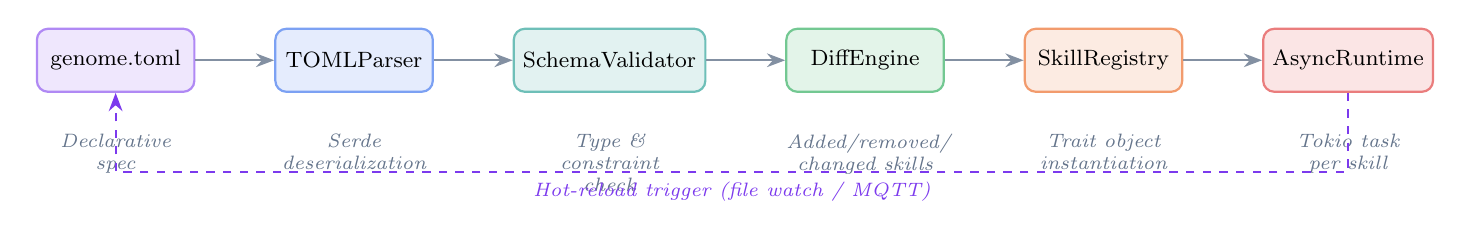
\begin{tikzpicture}[
    >=Stealth,
    node distance=0.5cm and 0.8cm,
    step/.style={draw, rounded corners=4pt, minimum width=2.0cm, minimum height=0.8cm, fill=#1!12, font=\footnotesize, text=black, draw=#1!60, thick},
    arrow/.style={->, thick, color=coregray!80},
    note/.style={font=\scriptsize\itshape, color=coregray, text width=2.0cm, align=center},
]

% Flow steps
\node[step=corepurple] (file) {genome.toml};
\node[step=coreblue, right=1.0cm of file] (parse) {TOML\\Parser};
\node[step=coreteal, right=1.0cm of parse] (validate) {Schema\\Validator};
\node[step=coregreen, right=1.0cm of validate] (diff) {Diff\\Engine};
\node[step=coreorange, right=1.0cm of diff] (registry) {Skill\\Registry};
\node[step=corered, right=1.0cm of registry] (runtime) {Async\\Runtime};

% Arrows
\draw[arrow] (file) -- (parse);
\draw[arrow] (parse) -- (validate);
\draw[arrow] (validate) -- (diff);
\draw[arrow] (diff) -- (registry);
\draw[arrow] (registry) -- (runtime);

% Notes below
\node[note, below=0.4cm of file] {Declarative\\spec};
\node[note, below=0.4cm of parse] {Serde\\deserialization};
\node[note, below=0.4cm of validate] {Type \&\\constraint check};
\node[note, below=0.4cm of diff] {Added/removed/\\changed skills};
\node[note, below=0.4cm of registry] {Trait object\\instantiation};
\node[note, below=0.4cm of runtime] {Tokio task\\per skill};

% Feedback loop
\draw[arrow, dashed, color=corepurple] (runtime.south) -- ++(0,-1.0) -| node[below, pos=0.25, font=\scriptsize\itshape, color=corepurple] {Hot-reload trigger (file watch / MQTT)} (file.south);

\end{tikzpicture}

\newpage

%% ========================================================================
%%  FIGURE 3: Genome Structure and Mutation Operators
%% ========================================================================

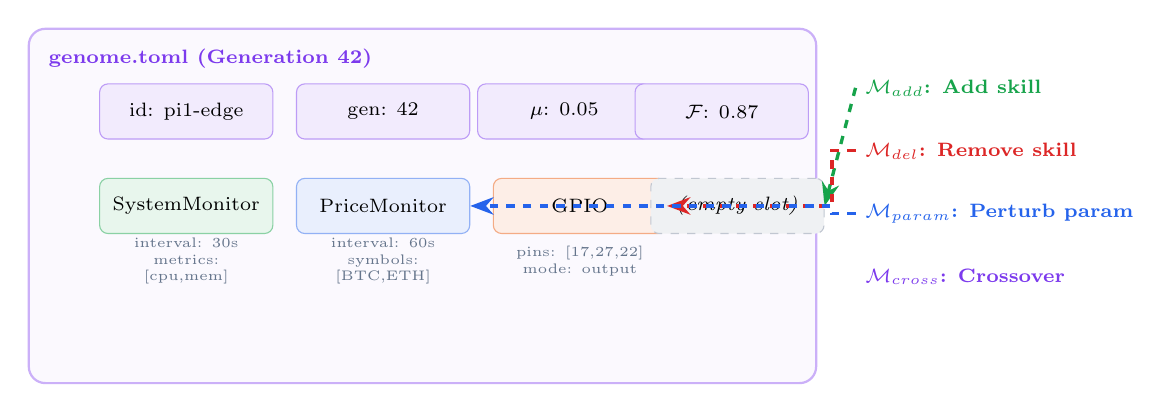
\begin{tikzpicture}[
    >=Stealth,
    block/.style={draw, rounded corners=3pt, minimum width=2.2cm, minimum height=0.7cm, font=\scriptsize, fill=#1!10, draw=#1!50},
    genome/.style={draw, rounded corners=6pt, minimum width=10cm, minimum height=4.5cm, fill=corepurple!3, draw=corepurple!40, thick},
    mutarrow/.style={->, very thick, color=#1, dashed},
    label/.style={font=\scriptsize\bfseries, color=#1},
]

% Genome container
\node[genome] (g) at (0,0) {};
\node[label=corepurple, anchor=north west] at ([xshift=4pt, yshift=-4pt]g.north west) {genome.toml (Generation 42)};

% Header section
\node[block=corepurple] (id) at (-3.0, 1.2) {id: pi1-edge};
\node[block=corepurple] (gen) at (-0.5, 1.2) {gen: 42};
\node[block=corepurple] (mu) at (1.8, 1.2) {$\mu$: 0.05};
\node[block=corepurple] (fit) at (3.8, 1.2) {$\mathcal{F}$: 0.87};

% Skills
\node[block=coregreen] (s1) at (-3.0, 0.0) {SystemMonitor};
\node[block=coreblue] (s2) at (-0.5, 0.0) {PriceMonitor};
\node[block=coreorange] (s3) at (2.0, 0.0) {GPIO};
\node[block=coregray, dashed, draw=coregray!40] (s4) at (4.0, 0.0) {\textit{(empty slot)}};

% Params under skills
\node[font=\tiny, text=coregray, text width=2cm, align=center] at (-3.0, -0.7) {interval: 30s\\metrics: [cpu,mem]};
\node[font=\tiny, text=coregray, text width=2cm, align=center] at (-0.5, -0.7) {interval: 60s\\symbols: [BTC,ETH]};
\node[font=\tiny, text=coregray, text width=2cm, align=center] at (2.0, -0.7) {pins: [17,27,22]\\mode: output};

% Mutation operators (outside genome)
\node[font=\scriptsize\bfseries, color=coregreen, anchor=west] (add) at (5.5, 1.5) {$\mathcal{M}_{\text{add}}$: Add skill};
\node[font=\scriptsize\bfseries, color=corered, anchor=west] (del) at (5.5, 0.7) {$\mathcal{M}_{\text{del}}$: Remove skill};
\node[font=\scriptsize\bfseries, color=coreblue, anchor=west] (param) at (5.5, -0.1) {$\mathcal{M}_{\text{param}}$: Perturb param};
\node[font=\scriptsize\bfseries, color=corepurple, anchor=west] (cross) at (5.5, -0.9) {$\mathcal{M}_{\text{cross}}$: Crossover};

% Mutation arrows
\draw[mutarrow=coregreen] (add.west) -- (s4.east);
\draw[mutarrow=corered] (del.west) -- +(-0.3,0) |- (s3.east);
\draw[mutarrow=coreblue] (param.west) -- +(-0.3,0) |- (s2.east);

\end{tikzpicture}

\newpage

%% ========================================================================
%%  FIGURE 4: Deployment Tiers
%% ========================================================================

\begin{tikzpicture}[
    >=Stealth,
    tier/.style={draw, rounded corners=6pt, minimum width=3.8cm, minimum height=3.5cm, fill=#1, thick, draw=#2},
    device/.style={draw, rounded corners=3pt, minimum width=3.0cm, minimum height=0.6cm, fill=white, font=\scriptsize, drop shadow={shadow xshift=0.3pt, shadow yshift=-0.3pt, opacity=0.1}},
    spec/.style={font=\tiny, color=coregray, text width=3.2cm, align=center},
    tierlab/.style={font=\small\bfseries, color=#1},
    conn/.style={<->, thick, color=coreteal, dashed},
]

% Edge Tier
\node[tier={edgebg}{coregreen!60}] (edge) at (-4.5, 0) {};
\node[tierlab=coregreen] at (-4.5, 2.0) {Edge Tier};
\node[device] at (-4.5, 1.2) {Raspberry Pi 1};
\node[device] at (-4.5, 0.4) {ESP32 / ARMv6};
\node[spec] at (-4.5, -0.4) {Binary: 3.0\,MB\\RAM: 3.2\,MB\\Skills: 1--5};
\node[spec] at (-4.5, -1.3) {Bare-metal\\Static linking\\No container};

% Server Tier
\node[tier={serverbg}{coreblue!60}] (server) at (0, 0) {};
\node[tierlab=coreblue] at (0, 2.0) {Server Tier};
\node[device] at (0, 1.2) {Podman Container};
\node[device] at (0, 0.4) {Docker / LXC};
\node[spec] at (0, -0.4) {Binary: 7.2\,MB\\RAM: 50--200\,MB\\Skills: 5--50};
\node[spec] at (0, -1.3) {Orchestrator\\100+ agents\\Auto-scaling};

% Cloud Tier
\node[tier={cloudbg}{coreorange!60}] (cloud) at (4.5, 0) {};
\node[tierlab=coreorange] at (4.5, 2.0) {Cloud Tier};
\node[device] at (4.5, 1.2) {E2B Sandbox};
\node[device] at (4.5, 0.4) {AWS / GCP VM};
\node[spec] at (4.5, -0.4) {RAM: 1--16\,GB\\Skills: unlimited\\Code exec};
\node[spec] at (4.5, -1.3) {Sandboxed\\Untrusted skills\\Ephemeral};

% Connections
\draw[conn] (edge.east) -- (server.west) node[midway, above, font=\tiny\bfseries, color=coreteal] {MQTT};
\draw[conn] (server.east) -- (cloud.west) node[midway, above, font=\tiny\bfseries, color=coreteal] {MQTT};

% Bottom label
\node[font=\footnotesize\itshape, color=coregray] at (0, -2.5) {Agents synchronize across all tiers via MQTT pub/sub with configurable QoS};

\end{tikzpicture}

\newpage

%% ========================================================================
%%  FIGURE 5: Skill Execution Timeline
%% ========================================================================

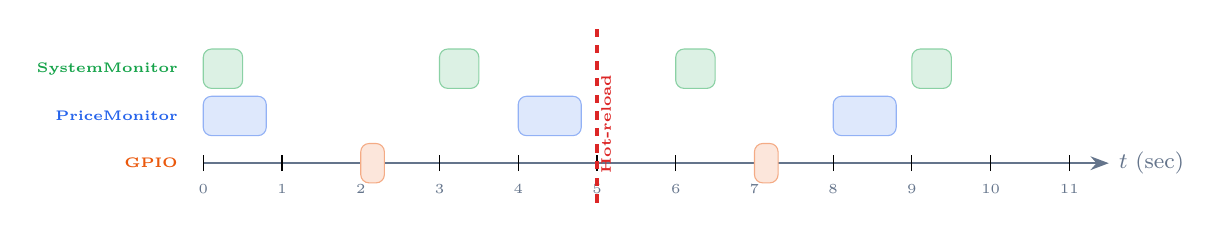
\begin{tikzpicture}[
    >=Stealth,
    task/.style={draw, rounded corners=3pt, minimum height=0.5cm, font=\tiny\ttfamily, fill=#1!15, draw=#1!50},
    timeline/.style={->, thick, color=coregray},
    tick/.style={font=\tiny, color=coregray},
]

% Time axis
\draw[timeline] (0, 0) -- (11.5, 0) node[right, font=\footnotesize] {$t$ (sec)};
\foreach \x in {0,1,...,11} {
    \draw (\x, -0.1) -- (\x, 0.1);
    \node[tick, below] at (\x, -0.15) {\x};
}

% Skill 1: SystemMonitor (every 3 ticks)
\node[font=\tiny\bfseries, color=coregreen, anchor=east] at (-0.2, 1.2) {SystemMonitor};
\foreach \x in {0, 3, 6, 9} {
    \node[task=coregreen, minimum width=0.5cm] at (\x+0.25, 1.2) {};
}

% Skill 2: PriceMonitor (every 4 ticks)
\node[font=\tiny\bfseries, color=coreblue, anchor=east] at (-0.2, 0.6) {PriceMonitor};
\foreach \x in {0, 4, 8} {
    \node[task=coreblue, minimum width=0.8cm] at (\x+0.4, 0.6) {};
}

% Skill 3: GPIO (event-driven)
\node[font=\tiny\bfseries, color=coreorange, anchor=east] at (-0.2, 0.0) {GPIO};
\node[task=coreorange, minimum width=0.3cm] at (2.15, 0.0) {};
\node[task=coreorange, minimum width=0.3cm] at (7.15, 0.0) {};

% Hot-reload event
\draw[very thick, color=corered, dashed] (5, -0.5) -- (5, 1.7);
\node[font=\tiny\bfseries, color=corered, rotate=90, anchor=south] at (5.3, 0.5) {Hot-reload};

\end{tikzpicture}

\newpage

%% ========================================================================
%%  FIGURE 6: Evolution Cycle (Bonus Figure)
%% ========================================================================

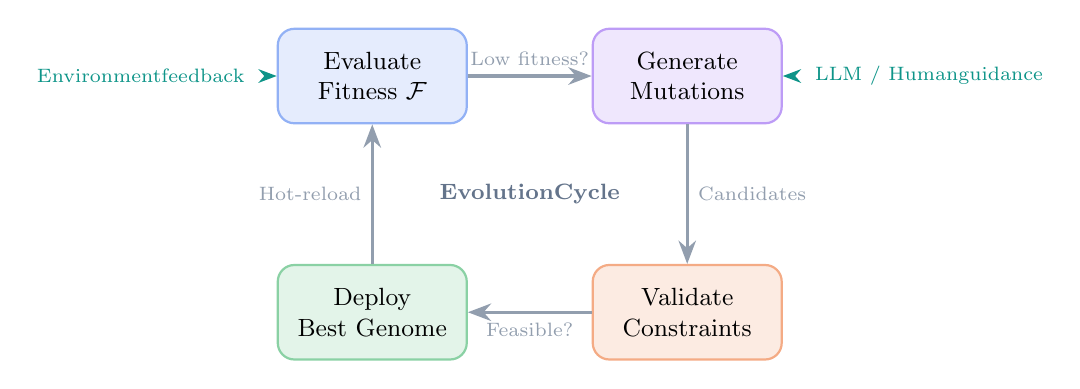
\begin{tikzpicture}[
    >=Stealth,
    phase/.style={draw, rounded corners=6pt, minimum width=2.4cm, minimum height=1.2cm, fill=#1!12, draw=#1!50, font=\small, thick, align=center},
    arrow/.style={->, very thick, color=coregray!70},
]

% Cycle nodes
\node[phase=coreblue] (eval) at (0, 3) {Evaluate\\Fitness $\mathcal{F}$};
\node[phase=corepurple] (mutate) at (4, 3) {Generate\\Mutations};
\node[phase=coreorange] (validate) at (4, 0) {Validate\\Constraints};
\node[phase=coregreen] (deploy) at (0, 0) {Deploy\\Best Genome};

% Arrows forming cycle
\draw[arrow] (eval) -- (mutate) node[midway, above, font=\scriptsize] {Low fitness?};
\draw[arrow] (mutate) -- (validate) node[midway, right, font=\scriptsize] {Candidates};
\draw[arrow] (validate) -- (deploy) node[midway, below, font=\scriptsize] {Feasible?};
\draw[arrow] (deploy) -- (eval) node[midway, left, font=\scriptsize] {Hot-reload};

% Center label
\node[font=\footnotesize\bfseries, color=coregray] at (2, 1.5) {Evolution\\Cycle};

% External inputs
\node[font=\scriptsize, color=coreteal, anchor=east] at (-1.5, 3) {Environment\\feedback};
\draw[->, color=coreteal, thick] (-1.3, 3) -- (eval.west);

\node[font=\scriptsize, color=coreteal, anchor=west] at (5.5, 3) {LLM / Human\\guidance};
\draw[->, color=coreteal, thick] (5.3, 3) -- (mutate.east);

\end{tikzpicture}

\end{document}
